% Architecture Design Template overview, derived from the Generic Slides template.
% Source diagrams are maintained in the corresponding DSN manual chapter.
\documentclass[aspectratio=169,11pt]{beamer}
% Matches the DSN manual version used by this presentation.
\newcommand{\TemplateVersion}{2.33}

\usepackage{beamerThemeSlides}
\usepackage{graphicx}
\usepackage{array}
\usepackage{booktabs}
\usepackage{pgfpages}
\usetikzlibrary{arrows.meta,calc,fit,positioning,shapes.geometric}
\ifdefined\InstructorNotes
  \setbeameroption{show notes on second screen=right}
\fi
\definecolor{dsnBlue}{RGB}{31,78,121}
\definecolor{dsnGreen}{RGB}{46,125,50}
\definecolor{dsnRed}{RGB}{183,28,28}
\definecolor{dsnGray}{RGB}{90,90,90}
\definecolor{dsnLightBlue}{RGB}{232,240,247}
\title{Architecture Design Template Slides}
\subtitle{A connected engineering record from need to release}
\author{Darian Muresan, Ph.D.}
\institute{Stevens Institute of Technology}
\date{October 2026}
\coursecode{DSN}
\hypersetup{pdftitle={Architecture Design Template Slides},pdfauthor={Darian Muresan},pdfsubject={Overview of the DSN architecture design template}}
\begin{document}
\SlideTitleFrame
\note{Present the deck as an overview of the DSN template, not as a completed project architecture. The manual remains the authoritative source.}

\begin{frame}{One maintained architecture record}
\begin{itemize}
  \item The template captures scope, requirements, design decisions, implementation, and evidence.
  \item Stable identifiers connect decisions to the need that motivated them and the tests that assess them.
  \item Each chapter supplies instructions and an example to replace with project facts.
\end{itemize}
\begin{slidecallout}{Use it as a decision record}
A claim in one chapter should be explainable and checkable through its links to other chapters.
\end{slidecallout}
\end{frame}
\note{Distinguish the template from a completed design. Its examples are placeholders; project owners must supply and review actual decisions and evidence.}

\begin{frame}{The V-model connects design and evidence}
\framesubtitle{Directly reused from Introduction, Figure 1.3}
\centering
\resizebox{!}{5.35cm}{% Adapted from MSE Figure 1.2; keep lifecycle and feedback routes orthogonal.
\begingroup
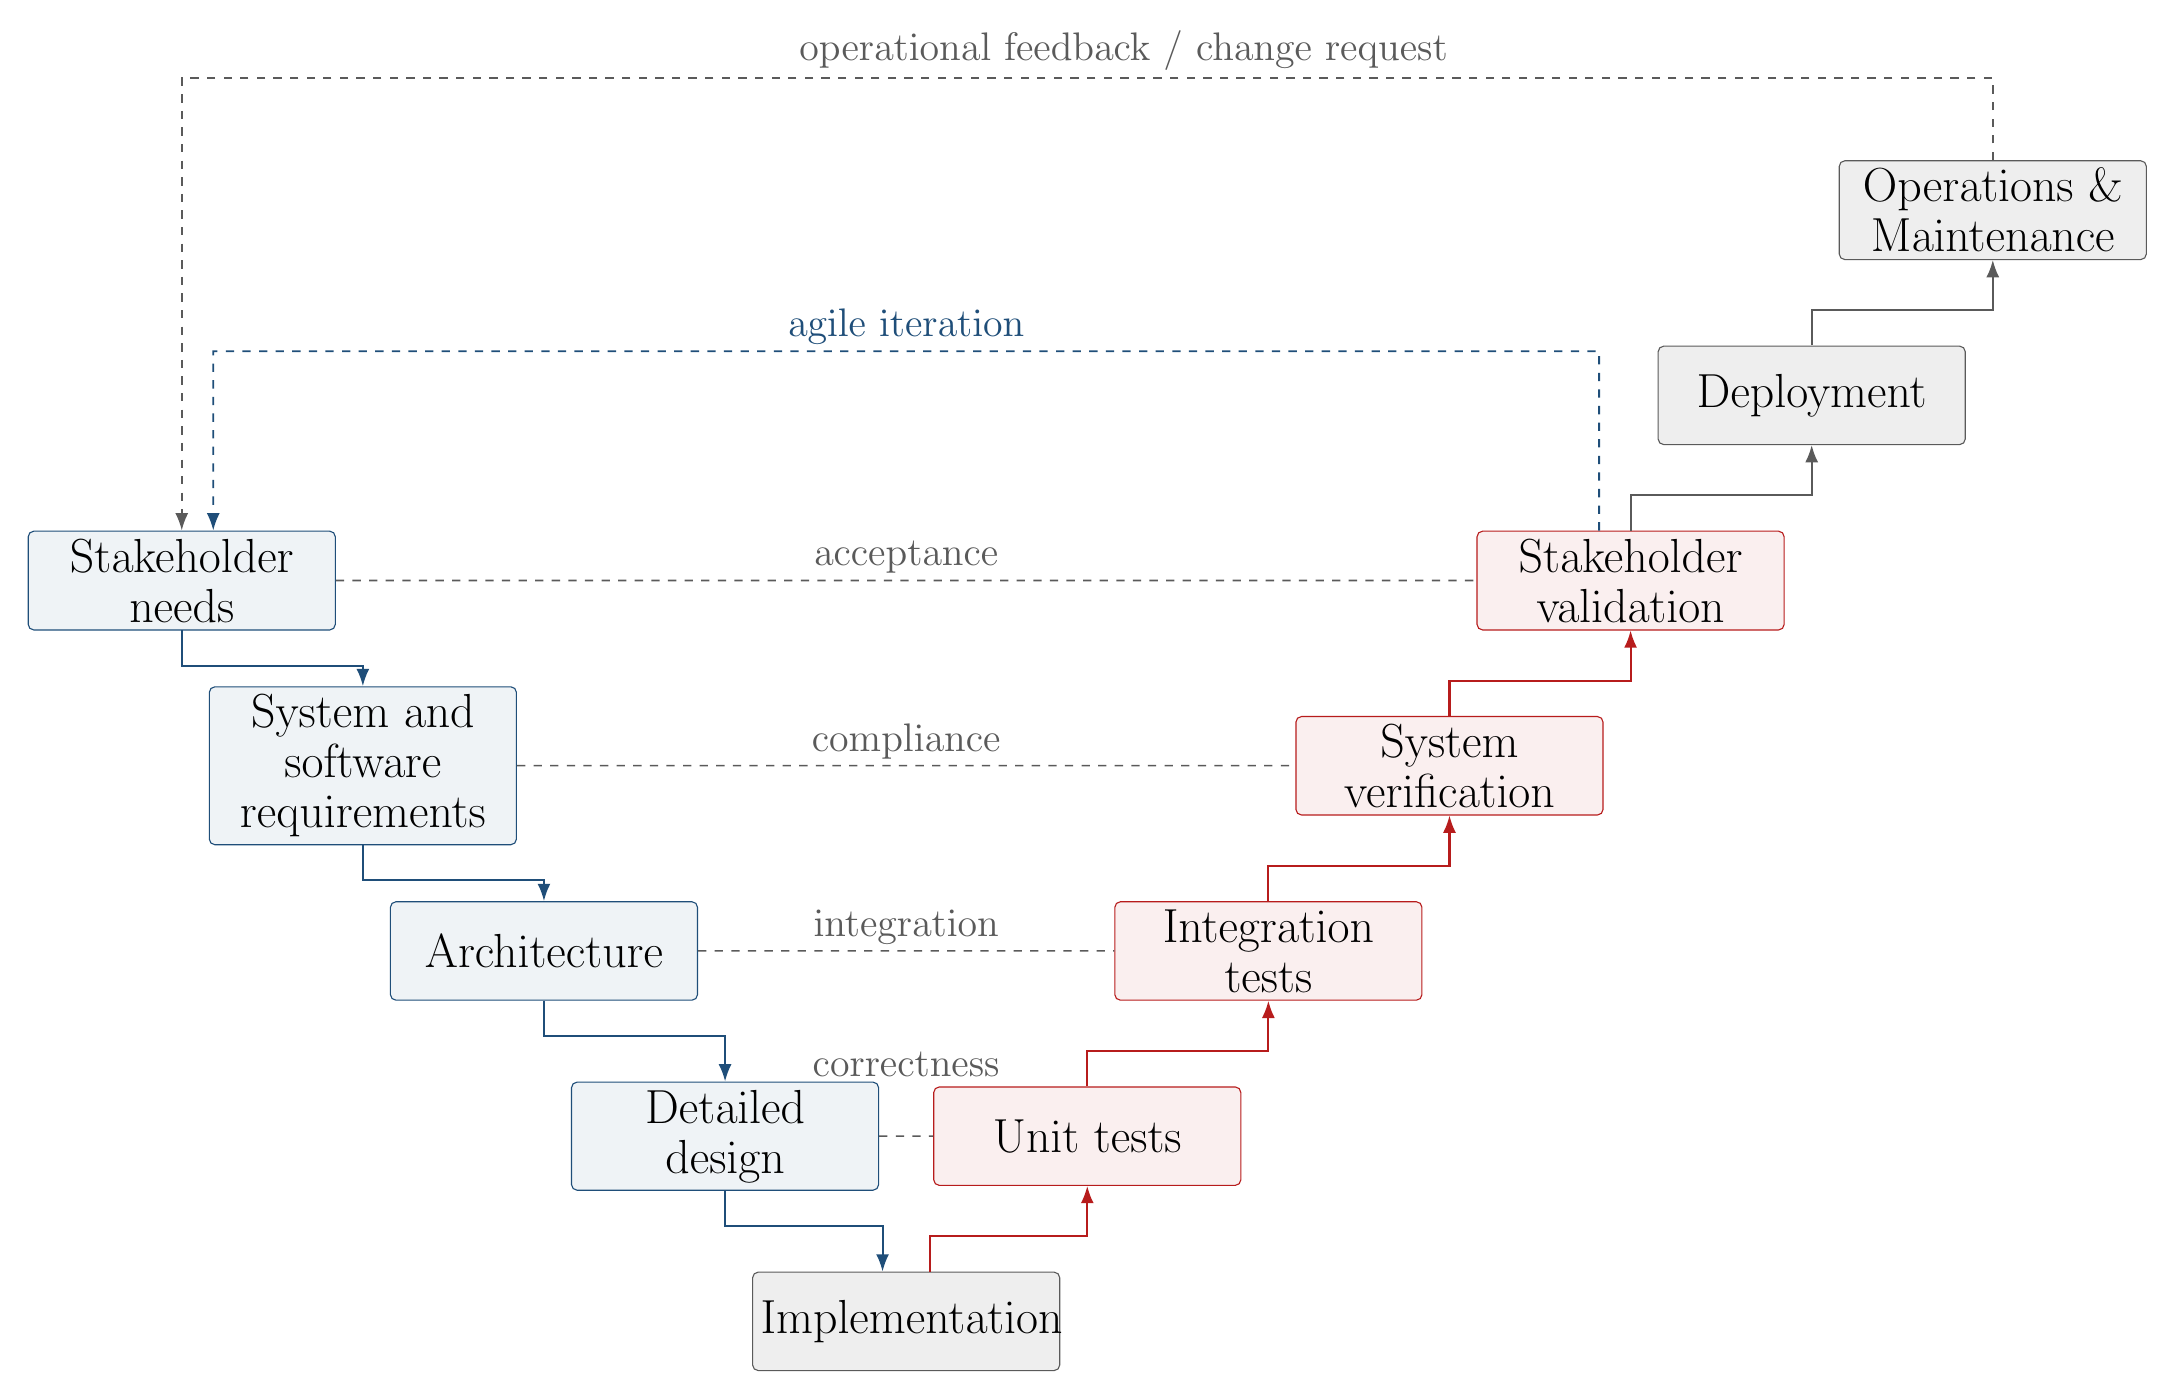
\begin{tikzpicture}[yscale=1.12,
  stage/.style={draw=dsnBlue,fill=dsnBlue!7,rounded corners=2pt,text width=3.7cm,inner sep=0.10cm,minimum width=3.9cm,minimum height=1.25cm,align=center,font=\fontsize{16}{18}\selectfont},
  evidence/.style={stage,draw=dsnRed,fill=dsnRed!7},
  implementation/.style={stage,draw=dsnGray,fill=dsnGray!10},
  operation/.style={stage,draw=dsnGray,fill=dsnGray!10},
  lifecycle/.style={-{Latex[length=2.2mm]},line width=0.75pt},
  relation/.style={draw=dsnGray,dashed,line width=0.6pt},
  feedback/.style={-{Latex[length=2.2mm]},draw=dsnGray,dashed,line width=0.7pt},
  label/.style={fill=white,inner sep=1.2pt,font=\fontsize{14}{16}\selectfont,text=dsnGray}
]
  \node[stage] (needs) at (-9.2,8.4) {Stakeholder needs};
  \node[stage] (requirements) at (-6.9,6.3) {System and software\\requirements};
  \node[stage] (architecture) at (-4.6,4.2) {Architecture};
  \node[stage] (design) at (-2.3,2.1) {Detailed design};
  \node[implementation] (implementation) at (0,0) {Implementation};
  \node[evidence] (unit) at (2.3,2.1) {Unit tests};
  \node[evidence] (integration) at (4.6,4.2) {Integration tests};
  \node[evidence] (verification) at (6.9,6.3) {System\\verification};
  \node[evidence] (validation) at (9.2,8.4) {Stakeholder\\validation};
  \node[operation] (deployment) at (11.5,10.5) {Deployment};
  \node[operation] (maintenance) at (13.8,12.6) {Operations \&\\ Maintenance};
  \draw[lifecycle,draw=dsnBlue] (needs.south) -- ++(0,-0.4) -| (requirements.north);
  \draw[lifecycle,draw=dsnBlue] (requirements.south) -- ++(0,-0.4) -| (architecture.north);
  \draw[lifecycle,draw=dsnBlue] (architecture.south) -- ++(0,-0.4) -| (design.north);
  \draw[lifecycle,draw=dsnBlue] (design.south) -- ++(0,-0.4) -| ([xshift=-3mm]implementation.north);
  \draw[lifecycle,draw=dsnRed] ([xshift=3mm]implementation.north) -- ++(0,0.4) -| (unit.south);
  \draw[lifecycle,draw=dsnRed] (unit.north) -- ++(0,0.4) -| (integration.south);
  \draw[lifecycle,draw=dsnRed] (integration.north) -- ++(0,0.4) -| (verification.south);
  \draw[lifecycle,draw=dsnRed] (verification.north) -- ++(0,0.4) -| (validation.south);
  \draw[lifecycle,draw=dsnGray] (validation.north) -- ++(0,0.4) -| (deployment.south);
  \draw[lifecycle,draw=dsnGray] (deployment.north) -- ++(0,0.4) -| (maintenance.south);
  \draw[feedback] (maintenance.north) -- (13.8,14.1)
    -- node[label,above=1pt,pos=0.48]{operational feedback / change request} (-9.2,14.1)
    -- (needs.north);
  \draw[relation] (needs) -- node[label,above=1pt]{acceptance} (validation);
  \draw[relation] (requirements) -- node[label,above=1pt]{compliance} (verification);
  \draw[relation] (architecture) -- node[label,above=1pt]{integration} (integration);
  \draw[relation] (design) -- node[label,above=20pt]{correctness} (unit);
  \draw[feedback,draw=dsnBlue] ([xshift=-4mm]validation.north)
    -- (8.8,11.0)
    -- node[label,above=1pt,text=dsnBlue]{agile iteration} (-8.8,11.0)
    -- ([xshift=4mm]needs.north);
\end{tikzpicture}
\endgroup
}
\end{frame}
\note{Walk down the left side from needs to implementation, then up the right side through tests and acceptance. Horizontal links state what each evidence level assesses. Point out agile iteration and operational feedback. The diagram source is shared with the manual.}

\begin{frame}{AI changes the execution loop}
\framesubtitle{The maintained inputs still define what is approved}
\centering
\resizebox{10.6cm}{!}{% Adapted from MSE Figure 2.1.
% Adapted from Week-02/TikZ/sldSourceOfTruthAnalogy/sldSourceOfTruthAnalogyDrawing.tex.
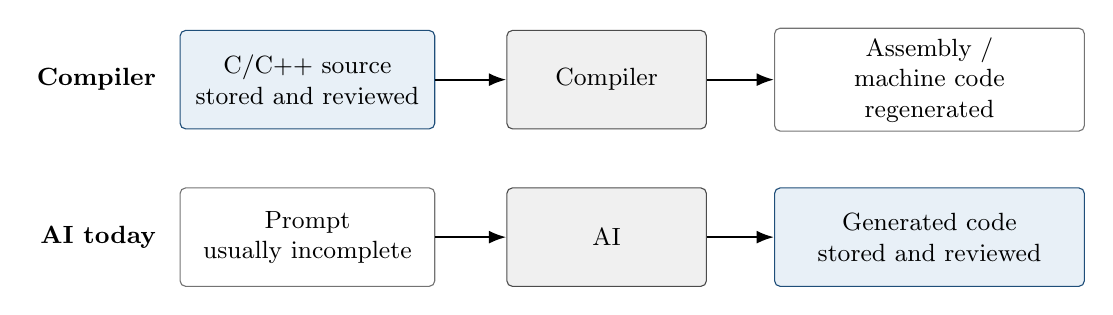
\begin{tikzpicture}[font=\small,
 source/.style={draw=dsnBlue,fill=dsnLightBlue,rounded corners=2pt,
   text width=3.0cm,minimum height=1.25cm,align=center},
 process/.style={draw=black!70,fill=black!6,rounded corners=2pt,
   text width=2.3cm,minimum height=1.25cm,align=center},
 output/.style={draw=black!55,rounded corners=2pt,
   text width=3.7cm,minimum height=1.25cm,align=center},
 arrow/.style={-{Latex[length=2.2mm]},line width=.8pt}]
\node[font=\small\bfseries,anchor=east] at (-1.1,0) {Compiler};
\node[source] (source) at (0.7,0) {C/C++ source\\stored and reviewed};
\node[process] (compiler) at (4.5,0) {Compiler};
\node[output] (binary) at (8.6,0) {Assembly /\\machine code\\regenerated};
\draw[arrow] (source) -- (compiler);
\draw[arrow] (compiler) -- (binary);
\node[font=\small\bfseries,anchor=east] at (-1.1,-2) {AI today};
\node[output,text width=3cm] (prompt) at (.7,-2) {Prompt\\usually incomplete};
\node[process] (ai) at (4.5,-2) {AI};
\node[source,text width=3.7cm] (code) at (8.6,-2) {Generated code\\stored and reviewed};
\draw[arrow] (prompt) -- (ai);
\draw[arrow] (ai) -- (code);
\end{tikzpicture}
}
\vspace{0.22cm}
\begin{slidecallout}{Architecture is an input}
An AI agent may propose a change; a human reviews its effect on requirements, design, tests, and release evidence.
\end{slidecallout}
\end{frame}
\note{This is Figure 1.1 in the DSN introduction, adapted from MSE Figure 2.1. Explain that generated code is reviewed, not treated as the sole maintained design source.}

\begin{frame}{Architecture updates close the AI loop}
\framesubtitle{Directly reused from Introduction, Figure 1.2}
\centering
\resizebox{11.0cm}{!}{% Adapted from MSE Figure 2.2.
% Adapted from Week-02/TikZ/sldArchitectureDirectsAI/sldArchitectureDirectsAIDrawing.tex.
% The two return routes share baseline approval, irrespective of who authors the update.
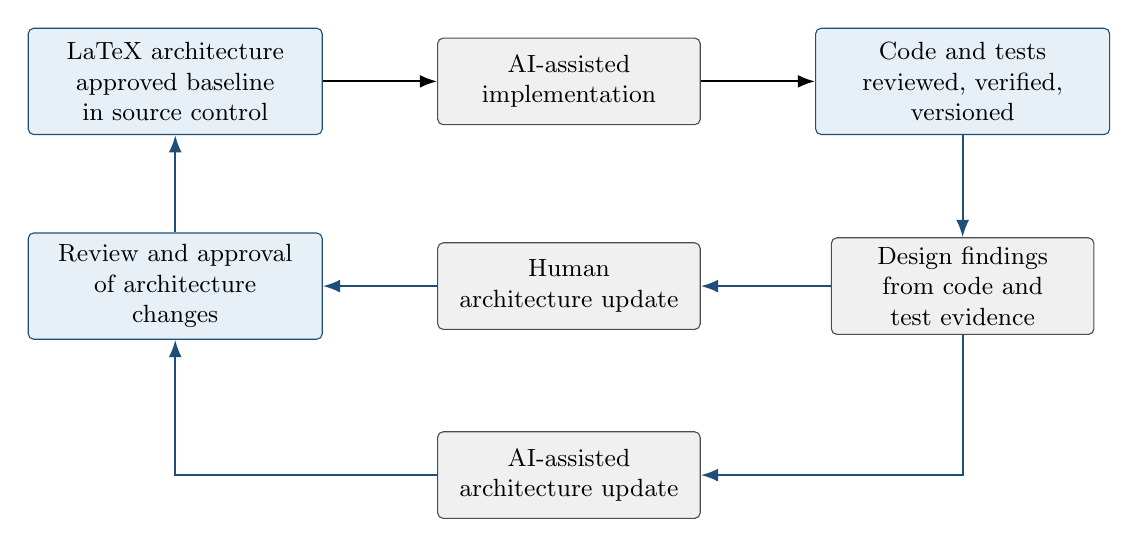
\begin{tikzpicture}[font=\small,
 source/.style={draw=dsnBlue,fill=dsnLightBlue,rounded corners=2pt,
   text width=3.5cm,minimum height=1.35cm,align=center},
 process/.style={draw=black!70,fill=black!6,rounded corners=2pt,
   text width=3.1cm,minimum height=1.1cm,align=center},
 arrow/.style={-{Latex[length=2.2mm]},line width=.8pt},
 feedback/.style={arrow,draw=dsnBlue}]
\node[source] (architecture) at (0,0)
 {LaTeX architecture\\approved baseline\\in source control};
\node[process] (implementation) at (5,0) {AI-assisted\\implementation};
\node[source] (code) at (10,0) {Code and tests\\reviewed, verified,\\versioned};
\draw[arrow] (architecture) -- (implementation);
\draw[arrow] (implementation) -- (code);
\node[process] (findings) at (10,-2.6) {Design findings\\from code and\\test evidence};
\node[process] (human) at (5,-2.6) {Human\\architecture update};
\node[process] (agent) at (5,-5) {AI-assisted\\architecture update};
\node[source] (review) at (0,-2.6) {Review and approval\\of architecture\\changes};
\draw[feedback] (code) -- (findings);
\draw[feedback] (findings) -- (human);
\draw[feedback] (human) -- (review);
\draw[feedback] (findings.south) |- (agent.east);
\draw[feedback] (agent.west) -| (review.south);
\draw[feedback] (review) -- (architecture);
\end{tikzpicture}
}
\end{frame}
\note{Describe the sequence: approved architecture and requirements enter the task; implementation and tests expose findings; a human approves changes to the baseline before another task uses it. The source figure belongs to the Introduction chapter.}

\begin{frame}{Linked evidence makes architecture navigable}
\begin{slidecallout}{Link to evidence wherever possible}
Use stable identifiers and hyperlinks so readers can follow a design claim to its rationale, implementation, and supporting results.
\end{slidecallout}
\begin{itemize}
  \item \textbf{Navigate directly:} link requirements, use cases, figures, tables, tests, and evidence to their authoritative definitions.
  \item \textbf{Trace in both directions:} follow a need toward its implementation and evidence; trace a result back to the need it supports.
  \item \textbf{Maintain one source:} reference authoritative artifacts and keep mappings in the traceability register.
\end{itemize}
\vspace{0.15cm}
\textbf{The architecture is a connected engineering record maintained like code.}
\end{frame}
\note{Sources: DSN Document Guide and Traceability chapters. Emphasize using linked evidence as much as possible to make navigation, impact analysis, and traceability easy. Stable IDs and hyperlinks connect the record; the canonical register records its mappings. Links help reviewers find evidence but do not establish that the evidence is sufficient or correct.}

\begin{frame}{Think of the template as code for architecture}
\begin{columns}[T,onlytextwidth]
\column{0.48\textwidth}
\begin{block}{A structured source project}
\begin{itemize}
  \item A main file assembles the manual.
  \item Chapter files separate responsibilities.
  \item Chapter folders hold editable TikZ diagrams.
  \item Build scripts produce the readable PDF.
\end{itemize}
\end{block}
\column{0.48\textwidth}
\begin{block}{A developer's workflow}
\begin{itemize}
  \item Record architecture artifacts in source control alongside the software.
  \item Review text and diagram changes as diffs.
  \item Update design, code, and linked evidence together.
  \item Rebuild and check links before baselining a revision.
\end{itemize}
\end{block}
\end{columns}
\vspace{0.2cm}
\textbf{The file structure organizes the architecture; revisions preserve how it evolves.}
\end{frame}
\note{The analogy is to a software source tree: the entry point includes responsibility-focused modules and shared assets, and a build produces a deliverable. Maintain the editable LaTeX and TikZ sources with the product revision. Record evidence versions and locations so links remain meaningful for that baseline. This is an authoring and configuration-management approach; the architecture itself is not executable software.}

\begin{frame}{The template has a software-style source structure}
\begin{columns}[T,onlytextwidth]
\column{0.50\textwidth}
\centering
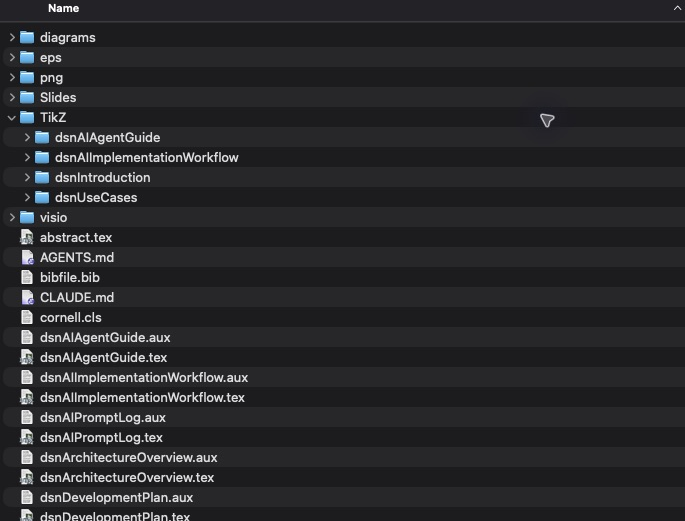
\includegraphics[width=\linewidth,height=5.0cm,keepaspectratio]{assets/dsnTemplateFileStructure.png}
\par\vspace{0.08cm}
{\scriptsize Actual DSN \texttt{main/} folder; Finder screenshot (excerpt).}
\column{0.47\textwidth}
\small
\textbf{Entry point}\par
\texttt{dsnManual.tex} assembles the chapters.
\vspace{0.18cm}

\textbf{Modules}\par
\texttt{dsnRequirements.tex}, \texttt{dsnLogicalView.tex}, etc. own chapter content.
\vspace{0.18cm}

\textbf{Shared diagram sources}\par
\texttt{TikZ/dsnIntroduction/}, etc. organize diagrams by chapter; slides reuse them.
\vspace{0.18cm}

\textbf{Build and presentation}\par
\texttt{makefileMacLinux} and \texttt{makefilePowerShell.ps1} build the manual; \texttt{Slides/} holds this deck.
\end{columns}
\end{frame}
\note{Screenshot captured from the actual ArchitectureDesignTemplate/main directory. It is cropped to the file list for legibility. This is an excerpt, not a complete directory inventory; the entry point and build scripts are elsewhere in the same directory. The .aux files visible in Finder are generated build intermediates. Editable chapter and TikZ sources remain authoritative, and the slide deck reuses the corresponding chapter diagrams.}

\begin{frame}{The manual follows the engineering path}
\small
\begin{columns}[T,onlytextwidth]
\column{0.48\textwidth}
\begin{block}{Define the system}
Development plan\\System context\\User stories, requirements, use cases
\end{block}
\begin{block}{Design the system}
Architecture overview\\User interface and logical, process, development, physical views
\end{block}
\column{0.48\textwidth}
\begin{block}{Build and assess}
Implementation and tests\\Traceability, verification, validation, release
\end{block}
\begin{block}{Govern the work}
Document guide and profiles\\AI agent guide and workflow\\History and evidence appendices
\end{block}
\end{columns}
\end{frame}
\note{Use this map to locate detailed instructions in the DSN manual. Chapters are ordered to make dependencies visible; iteration can revisit earlier chapters.}

\begin{frame}{Record the architecture at each revision}
\begin{itemize}
  \item \textbf{Version the document:} identify the architecture revision explicitly.
  \item \textbf{Maintain its history:} record the date, version, author, and change; link each entry to the affected content.
  \item \textbf{Check it in with the code:} preserve the architecture sources and linked evidence for the corresponding software revision.
\end{itemize}
\vspace{0.2cm}
\begin{slidecallout}{A record of the system at that point in time}
A shared revision shows the design, implementation status, and evidence that belong together.
\end{slidecallout}
\vspace{0.12cm}
{\small\textbf{Future direction:} A sufficiently complete architecture might one day support regenerating code instead of storing it.}
\end{frame}
\note{Sources: DSN Document History, Implementation, Traceability, and Introduction chapters. The version identifies the document; the history explains its evolution; source control preserves the corresponding artifact set. Check in editable LaTeX and TikZ sources with the software and preserve evidence versions or stable references. The future direction is a possibility, not a current template capability: replacing stored code would require reproducible generation, controlled tools and dependencies, and verification of the generated implementation.}

\begin{frame}{Organization makes the architecture usable}
\begin{itemize}
  \item \textbf{Give each chapter one responsibility:} state its purpose and expected result; keep definitions in their authoritative locations.
  \item \textbf{Keep AI instructions in the manual:} author them as \texttt{.tex} chapters so the compiled PDF provides contents, hyperlinks, and cross-references. Thin \texttt{.md} entry files point to that guidance.
  \item \textbf{Use UML wherever practical for software architecture:} choose diagrams that express structure, behavior, components, and deployment with consistent semantics.
  \item \textbf{Keep diagrams editable:} organize TikZ sources by chapter and link diagrams to the artifacts they describe.
\end{itemize}
\end{frame}
\note{Sources: DSN Document Authoring Guide, AI Agent Usage Guide, and architecture-view chapters. Organization is essential for finding and maintaining authoritative information. AI skill definitions and execution instructions live in LaTeX and are published as navigable parts of the manual; AGENTS.md, CLAUDE.md, and SKILL.md remain thin discovery pointers. UML is the preferred notation for software architecture wherever it fits the question. TikZ is the editable drawing source, not a substitute for UML semantics.}

\begin{frame}{Introduction}
\framesubtitle{Chapter 1}
\begin{block}{Responsibility}
Establish the purpose, scope, audience, and conventions of the engineering record.
\end{block}
\begin{itemize}
  \item Define what the system and document cover, including exclusions and constraints.
  \item Explain the V-model, maintained design sources, and the role of AI assistance.
  \item Set the terminology and tailoring approach used throughout the manual.
  \item Explain how to instantiate a new project from the template.
\end{itemize}
\vspace{0.15cm}
\textbf{Expected result:} A shared understanding of how to read and use the architecture.
\end{frame}
\note{Source: Introduction chapter (dsnIntroduction.tex). Explain how this chapter contributes to the connected engineering record. Establish the purpose, scope, audience, and conventions of the engineering record. Point out the section Initializing a New Project from This Template.}

\begin{frame}{Development Plan}
\framesubtitle{Chapter 2}
\begin{block}{Responsibility}
Define how the project is governed, planned, reviewed, and changed.
\end{block}
\begin{itemize}
  \item Assign roles, milestones, review gates, and approval responsibilities.
  \item Record risks and the process for controlling changes.
  \item Decide domain-profile applicability with rationale, owner, and decision date.
\end{itemize}
\vspace{0.15cm}
\textbf{Expected result:} An actionable plan with visible ownership and decision gates.
\end{frame}
\note{Source: DevelopmentPlan chapter (dsnDevelopmentPlan.tex). Explain how this chapter contributes to the connected engineering record. Define how the project is governed, planned, reviewed, and changed.}

\begin{frame}{System Context}
\framesubtitle{Chapter 3}
\begin{block}{Responsibility}
Define the system boundary and its relationship to the surrounding environment.
\end{block}
\begin{itemize}
  \item Describe the problem, stakeholders, external actors, and external systems.
  \item Identify interfaces, exchanged information, and interface ownership.
  \item Record assumptions, dependencies, and exclusions.
\end{itemize}
\vspace{0.15cm}
\textbf{Expected result:} An agreed boundary for requirements and design decisions.
\end{frame}
\note{Source: SystemContext chapter (dsnSystemContext.tex). Explain how this chapter contributes to the connected engineering record. Define the system boundary and its relationship to the surrounding environment.}

\begin{frame}{User Stories}
\framesubtitle{Chapter 4}
\begin{block}{Responsibility}
Capture who needs a result and why that result has value.
\end{block}
\begin{itemize}
  \item Identify the beneficiary, desired outcome, priority, and acceptance criteria.
  \item Give each story a stable US identifier.
  \item Link stakeholder intent to the requirements that realize it.
\end{itemize}
\vspace{0.15cm}
\textbf{Expected result:} A reviewable statement of stakeholder value and acceptance intent.
\end{frame}
\note{Source: UserStories chapter (dsnUserStories.tex). Explain how this chapter contributes to the connected engineering record. Capture who needs a result and why that result has value.}

\begin{frame}{Requirements}
\framesubtitle{Chapter 5: a foundation for design, implementation, and verification}
\begin{block}{Responsibility}
Capture all applicable obligations for the system and its development in a verifiable form.
\end{block}
\begin{itemize}
  \item \textbf{Classify by purpose:} functional (what it does), quality / non-functional (how well), and constraints (binding limits).
  \item \textbf{Slice the requirements package:} use business, interface, security, and data families; filter by subsystem, quality subtype, priority, status, or version. Keep one authoritative requirement and link across views.
  \item Write singular, verifiable requirements with stable IDs. Use the registers, including priority, status, and \textbf{In Version}; link use cases and tests.
\end{itemize}
\vspace{0.1cm}
\textbf{Expected result:} A controlled set of obligations that can be implemented and assessed.
\end{frame}
\note{Source: Requirements chapter (dsnRequirements.tex), especially the identifier convention, functional and quality distinction, and category catalog. Families and review views are adaptable; each requirement has one primary register and a stable identifier. Specialized registers may include both functional and quality obligations. Filter or link rather than copying requirements. Leave In Version unassigned until implementation is complete in a controlled version.}

\begin{frame}{The full scope of requirements}
\framesubtitle{Chapter 5: one of the most important chapters}
\begin{itemize}
  \item \textbf{Include all types of requirements:} the chapter extends beyond the usual functional, quality, business, interface, security, and data requirements.
  \item \textbf{Developer requirements:} coding conventions, tools, build environments, testing practices, and development workflows.
  \item \textbf{AI requirements:} agent instructions, permitted actions, human review, and required evidence.
  \item \textbf{Naming requirements:} namespaces, class names, identifiers, files, and document conventions.
  \item \textbf{All applicable constraints:} technology, platforms, standards, regulation, resources, schedule, budget, and organizational policies.
\end{itemize}
\vspace{0.1cm}
{\small\textbf{Tailor to the domain:} Use template tailoring profiles to customize requirements---for example, embedded systems may add timing, memory, power, and hardware constraints.}
\end{frame}
\note{Sources for tailoring: Introduction, Template Tailoring and Domain Profiles; Requirements, Domain Profile Impact on Requirements. Evaluate each applicable profile and turn relevant concerns into project requirements or links to existing requirements, with documented exclusions. Embedded timing, memory, power, and hardware constraints are illustrative concerns, not automatically applicable obligations. The breadth of this chapter is emphasized at the user's direction. Requirements may govern the product, its developers, AI agents, and the engineering process. These examples are concerns to capture, not new requirement identifier families. Reuse the template's defined families according to the primary obligation; follow its approval convention before introducing a family or scope code. Detailed AI, naming, and authoring guidance can remain in its authoritative chapter and be referenced from the requirements package without duplicating it.}

\begin{frame}{Quality subtypes and scenarios}
\framesubtitle{Chapter 5: prompts for design decisions}
\begin{itemize}
  \item \textbf{Use subtypes to prompt questions:} performance and capacity; reliability and recovery; security and privacy; usability and accessibility; maintainability and testability; portability and interoperability.
  \item \textbf{Ask what the system must handle:} peak load, failures, threats, different users, future changes, and external dependencies. Define measurable conditions and success criteria.
  \item \textbf{Optional extension: quality scenarios.} Describe the stimulus, operating conditions, affected part of the system, expected response, and measurable outcome.
  \item Reference scenarios from the \textbf{requirements package}; link them to the relevant requirement IDs, design decisions, and tests.
\end{itemize}
\vspace{0.1cm}
{\small\textbf{Example --- recoverability:} During acquisition, a connection fails; reconnect within 5 seconds and report any lost samples.}
\end{frame}
\note{Source for quality subtypes: the Requirements chapter category catalog. This list prompts consideration; select applicable concerns and justify omissions. Quality scenarios are an optional extension proposed for this presentation, not an existing scenario register in the template. Give each scenario a stable reference in the requirements package and link it to measurable quality requirements and verification evidence. The recovery example is illustrative, not a project requirement or an agreed threshold. A fuller scenario can identify the stimulus source, stimulus, environment, affected artifact, response, and response measure.}

\begin{frame}{Use Cases}
\framesubtitle{Chapter 6}
\begin{block}{Responsibility}
Describe how actors interact with the system to achieve their goals.
\end{block}
\begin{itemize}
  \item Show actors and goals inside a clear UML system boundary.
  \item Give each UC identifier its own standard use-case table.
  \item Record triggers, preconditions, main and alternate flows, outcomes, and links.
\end{itemize}
\vspace{0.15cm}
\textbf{Expected result:} Complete interaction scenarios tied to requirements and tests.
\end{frame}
\note{Source: UseCases chapter (dsnUseCases.tex). Explain how this chapter contributes to the connected engineering record. Describe how actors interact with the system to achieve their goals.}

\begin{frame}{Architecture Overview}
\framesubtitle{Chapter 7}
\begin{block}{Responsibility}
Explain the major design choices and why they address the design drivers.
\end{block}
\begin{itemize}
  \item Identify driving requirements, quality attributes, constraints, and risks.
  \item Compare alternatives and record decisions, rationale, and consequences.
  \item Introduce the architecture views and the question each view answers.
\end{itemize}
\vspace{0.15cm}
\textbf{Expected result:} A defensible design direction with explicit trade-offs.
\end{frame}
\note{Source: ArchitectureOverview chapter (dsnArchitectureOverview.tex). Explain how this chapter contributes to the connected engineering record. Explain the major design choices and why they address the design drivers.}

\begin{frame}{User Interface Design}
\framesubtitle{Chapter 8}
\begin{block}{Responsibility}
Define how people interact with the system and understand its state.
\end{block}
\begin{itemize}
  \item Describe users, screens, workflows, and navigation.
  \item Specify feedback, accessibility, and essential interaction states.
  \item Use prototypes where they resolve uncertainty about behavior.
\end{itemize}
\vspace{0.15cm}
\textbf{Expected result:} An interaction design that supports stakeholder tasks and acceptance.
\end{frame}
\note{Source: UserInterfaceDesign chapter (dsnUserInterfaceDesign.tex). Explain how this chapter contributes to the connected engineering record. Define how people interact with the system and understand its state.}

\begin{frame}{Logical View}
\framesubtitle{Chapter 9}
\begin{block}{Responsibility}
Define the concepts, classes, interfaces, and responsibilities of the design.
\end{block}
\begin{itemize}
  \item Show relationships, data ownership, and important invariants.
  \item List primary class and interface responsibilities in a titled, labeled register.
  \item Keep diagram names, register entries, and links consistent.
\end{itemize}
\vspace{0.15cm}
\textbf{Expected result:} A structural model with explicit responsibility and ownership.
\end{frame}
\note{Source: LogicalView chapter (dsnLogicalView.tex). Explain how this chapter contributes to the connected engineering record. Define the concepts, classes, interfaces, and responsibilities of the design.}

\begin{frame}{Process View}
\framesubtitle{Chapter 10}
\begin{block}{Responsibility}
Explain how the system behaves while it is running.
\end{block}
\begin{itemize}
  \item Describe workflows, concurrency, synchronization, and state changes.
  \item Show significant interactions using UML activity, sequence, or state diagrams.
  \item Include failure paths and recovery behavior where they affect the design.
\end{itemize}
\vspace{0.15cm}
\textbf{Expected result:} A runtime model that explains coordination and observable behavior.
\end{frame}
\note{Source: ProcessView chapter (dsnProcessView.tex). Explain how this chapter contributes to the connected engineering record. Explain how the system behaves while it is running.}

\begin{frame}{Development View}
\framesubtitle{Chapter 11}
\begin{block}{Responsibility}
Map the design to source organization and build artifacts.
\end{block}
\begin{itemize}
  \item Identify modules, services, libraries, and their implementation boundaries.
  \item Define allowed dependencies and the rules that preserve those boundaries.
  \item Explain how source units form the deliverable artifacts.
\end{itemize}
\vspace{0.15cm}
\textbf{Expected result:} A code organization that developers can implement consistently.
\end{frame}
\note{Source: DevelopmentView chapter (dsnDevelopmentView.tex). Explain how this chapter contributes to the connected engineering record. Map the design to source organization and build artifacts.}

\begin{frame}{Physical View}
\framesubtitle{Chapter 12}
\begin{block}{Responsibility}
Describe where the system runs and how deployed elements communicate.
\end{block}
\begin{itemize}
  \item Use UML deployment diagrams for nodes, execution environments, and artifacts.
  \item Identify networks, data stores, trust boundaries, and runtime dependencies.
  \item Record operational constraints, monitoring, availability, and recovery ownership.
\end{itemize}
\vspace{0.15cm}
\textbf{Expected result:} A deployment model grounded in the operating environment.
\end{frame}
\note{Source: PhysicalView chapter (dsnPhysicalView.tex). Explain how this chapter contributes to the connected engineering record. Describe where the system runs and how deployed elements communicate.}

\begin{frame}{Implementation}
\framesubtitle{Chapter 13}
\begin{block}{Responsibility}
Make the architecture reproducible through concrete implementation guidance.
\end{block}
\begin{itemize}
  \item Record the technology baseline and required configuration.
  \item Provide the build and run commands.
  \item Define coding conventions and completion criteria that enforce the design.
\end{itemize}
\vspace{0.15cm}
\textbf{Expected result:} A repeatable path from design to a working implementation.
\end{frame}
\note{Source: Implementation chapter (dsnImplementation.tex). Explain how this chapter contributes to the connected engineering record. Make the architecture reproducible through concrete implementation guidance.}

\begin{frame}{Tests}
\framesubtitle{Chapter 14}
\begin{block}{Responsibility}
Define repeatable procedures that produce objective evidence.
\end{block}
\begin{itemize}
  \item Assign stable TC identifiers and map tests to requirements.
  \item Specify environments, inputs, entry conditions, steps, and expected results.
  \item Define how execution results and evidence are recorded.
\end{itemize}
\vspace{0.15cm}
\textbf{Expected result:} Executable test specifications with observable pass criteria.
\end{frame}
\note{Source: Tests chapter (dsnTests.tex). Explain how this chapter contributes to the connected engineering record. Define repeatable procedures that produce objective evidence.}

\begin{frame}{Traceability}
\framesubtitle{Chapter 15}
\begin{block}{Responsibility}
Maintain the canonical links from stakeholder need to release evidence.
\end{block}
\begin{itemize}
  \item Connect stories, requirements, use cases, tests, verification, and validation.
  \item Trace design decisions and implementation through the engineering record.
  \item Review missing backward and forward links and keep reciprocal mappings aligned.
\end{itemize}
\vspace{0.15cm}
\textbf{Expected result:} Visible coverage and identifiable gaps across the lifecycle.
\end{frame}
\note{Source: Traceability chapter (dsnTraceability.tex). Explain how this chapter contributes to the connected engineering record. Maintain the canonical links from stakeholder need to release evidence.}

\begin{frame}{Verification}
\framesubtitle{Chapter 16}
\begin{block}{Responsibility}
Show that each requirement conforms to its specification.
\end{block}
\begin{itemize}
  \item Select test, inspection, analysis, or demonstration as the verification method.
  \item Record VER identifiers, evidence references, reviewer, result, and any waiver.
  \item Support each compliance conclusion with controlled evidence.
\end{itemize}
\vspace{0.15cm}
\textbf{Expected result:} A requirement-by-requirement account of demonstrated compliance.
\end{frame}
\note{Source: Verification chapter (dsnVerification.tex). Explain how this chapter contributes to the connected engineering record. Show that each requirement conforms to its specification.}

\begin{frame}{Validation}
\framesubtitle{Chapter 17}
\begin{block}{Responsibility}
Show that the completed system meets stakeholder needs in its intended context.
\end{block}
\begin{itemize}
  \item Define realistic scenarios, participant roles, and success criteria.
  \item Record observations and results under stable VAL identifiers.
  \item Link outcomes to user stories and disposition issues or required changes.
\end{itemize}
\vspace{0.15cm}
\textbf{Expected result:} Evidence that stakeholders can achieve their intended outcomes.
\end{frame}
\note{Source: Validation chapter (dsnValidation.tex). Explain how this chapter contributes to the connected engineering record. Show that the completed system meets stakeholder needs in its intended context.}

\begin{frame}{Release}
\framesubtitle{Chapter 18}
\begin{block}{Responsibility}
Identify the exact deliverable and establish its readiness for authorized release.
\end{block}
\begin{itemize}
  \item Record versions, package contents, artifact identities, and known limitations.
  \item Link tests, verification, validation, approvals, and approved waivers.
  \item Describe deployment, rollback, recovery, and support arrangements.
\end{itemize}
\vspace{0.15cm}
\textbf{Expected result:} A controlled release package presented to the release authority.
\end{frame}
\note{Source: Release chapter (dsnRelease.tex). Explain how this chapter contributes to the connected engineering record. Identify the exact deliverable and establish its readiness for authorized release.}

\begin{frame}{Document Authoring Guide}
\framesubtitle{Appendix A}
\begin{block}{Responsibility}
Keep the manual consistent, maintainable, and reproducible.
\end{block}
\begin{itemize}
  \item Define file naming, namespaces, LaTeX conventions, and the build process.
  \item Require stable references and titles for figures, tables, and registers.
  \item Maintain editable diagram sources and inspect the rendered document.
\end{itemize}
\vspace{0.15cm}
\textbf{Expected result:} An engineering document whose sources and references remain usable.
\end{frame}
\note{Source: DocumentGuide chapter (dsnDocumentGuide.tex). Explain how this chapter contributes to the connected engineering record. Keep the manual consistent, maintainable, and reproducible.}

\begin{frame}{Embedded Systems Tailoring Profile}
\framesubtitle{Appendix B}
\begin{block}{Responsibility}
Add the concerns needed when software interacts with constrained hardware.
\end{block}
\begin{itemize}
  \item Record profile applicability in the Development Plan.
  \item Address hardware/software allocation, timing, resource budgets, and interfaces.
  \item Carry safety, security, toolchain, and hardware-test concerns into core chapters.
\end{itemize}
\vspace{0.15cm}
\textbf{Expected result:} The core architecture tailored to the embedded operating context.
\end{frame}
\note{Source: EmbeddedSystemsProfile chapter (dsnEmbeddedSystemsProfile.tex). Explain how this chapter contributes to the connected engineering record. Add the concerns needed when software interacts with constrained hardware.}

\begin{frame}{AI Agent Usage Guide}
\framesubtitle{Appendix C}
\begin{block}{Responsibility}
Define the authoritative inputs and acceptance criteria for AI-assisted tasks.
\end{block}
\begin{itemize}
  \item Use the AI Skills Register to select task context, steps, and acceptance criteria.
  \item Apply source-of-truth rules, consistent terminology, and human decision boundaries.
  \item Route each task to the chapters and evidence needed to perform it.
\end{itemize}
\vspace{0.15cm}
\textbf{Expected result:} A bounded task specification that an AI agent can follow and review.
\end{frame}
\note{Source: AIAgentGuide chapter (dsnAIAgentGuide.tex). Explain how this chapter contributes to the connected engineering record. Define the authoritative inputs and acceptance criteria for AI-assisted tasks.}

\begin{frame}{AI-Assisted Execution Workflow}
\framesubtitle{Appendix D}
\begin{block}{Responsibility}
Organize AI-assisted work from planning through integration and human review.
\end{block}
\begin{itemize}
  \item Plan, assign, execute, integrate, check, and review the selected AI Skills.
  \item Choose one or more agents only when tools, authorization, and task structure permit.
  \item Control file ownership, correction attempts, evidence, and the review handoff.
\end{itemize}
\vspace{0.15cm}
\textbf{Expected result:} Coordinated execution with explicit checks and approval boundaries.
\end{frame}
\note{Source: AIImplementationWorkflow chapter (dsnAIImplementationWorkflow.tex). Explain how this chapter contributes to the connected engineering record. Organize AI-assisted work from planning through integration and human review.}

\begin{frame}{AI Prompt Log}
\framesubtitle{Appendix E}
\begin{block}{Responsibility}
Preserve the provenance of material AI assistance and its human review.
\end{block}
\begin{itemize}
  \item Record date, tool or model, inputs, task, and generated output.
  \item Document review, corrections, and unresolved assumptions.
  \item Record proposed requirement-code extensions and their approval or rejection.
\end{itemize}
\vspace{0.15cm}
\textbf{Expected result:} An auditable account of how AI contributed to the engineering record.
\end{frame}
\note{Source: AIPromptLog chapter (dsnAIPromptLog.tex). Explain how this chapter contributes to the connected engineering record. Preserve the provenance of material AI assistance and its human review.}

\begin{frame}{Test Evidence}
\framesubtitle{Appendix F}
\begin{block}{Responsibility}
Retain detailed evidence supporting test and verification conclusions.
\end{block}
\begin{itemize}
  \item Store or link reports, logs, screenshots, and other execution artifacts.
  \item Identify the test, result, environment, date, and product revision.
  \item Keep evidence readable, traceable, and appropriately redacted.
\end{itemize}
\vspace{0.15cm}
\textbf{Expected result:} Accessible evidence behind the results summarized in the main chapters.
\end{frame}
\note{Source: TestEvidence chapter (dsnTestEvidence.tex). Explain how this chapter contributes to the connected engineering record. Retain detailed evidence supporting test and verification conclusions.}

\begin{frame}{Document History}
\framesubtitle{Appendix G}
\begin{block}{Responsibility}
Preserve the approved evolution of the architecture document.
\end{block}
\begin{itemize}
  \item Record the date, version, author, change, and rationale.
  \item Link each entry to the affected chapter, section, table, figure, or artifact.
  \item Keep approved entries and place the newest approved change first.
\end{itemize}
\vspace{0.15cm}
\textbf{Expected result:} A durable record of what changed, why, and where.
\end{frame}
\note{Source: DocumentHistory chapter (dsnDocumentHistory.tex). Explain how this chapter contributes to the connected engineering record. Preserve the approved evolution of the architecture document.}

\SlideSectionFrame[Customize the architecture for a specific project]{How to use\\the template}
\note{Transition from the chapter responsibilities to applying the template. The following slides describe initialization, project boundaries, requirements, design, evidence, and tailoring.}

\begin{frame}{Initialize a project with an AI agent}
\framesubtitle{Manual Section 1.9: Initializing a New Project from This Template}
{\small Open the project copy in your AI tool, attach the available project evidence, and replace \mbox{\texttt{[Project Name]}}. Enter:\par}
\vspace{0.2cm}
\begingroup\small\ttfamily\raggedright
\noindent Read dsnAIAgentGuide.tex and use the AIS-02 task steps for [Project Name]. Execute using Appendix D. Review the supplied project evidence and create a gap list before editing. Identify missing scope, stakeholders, interfaces, constraints, quality attributes, risks, evidence, and approvals. Identify the available domain profiles and ask me to confirm whether each is Applicable, Not Applicable, or TBD. Read each Applicable or relevant TBD profile and add its concerns to the gap list. After the gap list is reviewed, replace only supported placeholders and develop the document in dependency order. Compile the complete PDF and report unresolved human decisions.\par
\endgroup
\vspace{0.2cm}
{\small\textbf{Be ready to supply:} the project namespace, metadata, profile decisions, and missing evidence.}
\end{frame}
\note{Sources: Introduction Section 1.9 (Section:InitializeNewProject) and AI Agent Guide, Initialize the Architecture Book (Section:AIInitializePrompt). The displayed request reproduces the manual's initialization prompt. Start with a project copy of the template and provide the AI tool access to that workspace and supplied evidence. Appendix D is the AI Implementation Workflow. AIS-02 requires a human-confirmed namespace before creating or renaming files and recorded profile applicability decisions. Review the gap list before detailed work; unsupported facts remain gaps.}

\begin{frame}{Begin with the system boundary}
\begin{itemize}
  \item Name the system, stakeholders, external actors, and neighboring systems.
  \item State what is inside the boundary and what remains an external dependency.
  \item Record assumptions, constraints, data exchanged, and failure behavior.
\end{itemize}
\begin{slidecallout}{First review question}
Could a new team member tell which team owns each interface and behavior?
\end{slidecallout}
\end{frame}
\note{Point the audience to System Context before discussing internals. The boundary limits both requirements and architecture claims.}

\begin{frame}{Translate needs into assessable obligations}
\small
\begin{tabular}{@{}p{0.24\textwidth}p{0.63\textwidth}@{}}
\toprule
Artifact & Question it answers \\
\midrule
User story & Who needs a result, and why? \\
Use case & What interaction reaches that result, including alternatives? \\
Requirement & What behavior or quality must be satisfied? \\
Acceptance criteria & What observable result would count as success? \\
\bottomrule
\end{tabular}
\vspace{0.3cm}
\begin{slidecallout}{Keep links explicit}
Use IDs such as \texttt{US-001}, \texttt{UC-001}, and \texttt{REQ-F-001}.
\end{slidecallout}
\end{frame}
\note{Explain that prose alone is insufficient. Requirements need implementation versions, status, and references in the template registers. Use cases use the template's standard use-case table.}

\begin{frame}{Record decisions and their consequences}
\begin{itemize}
  \item Identify a decision as \texttt{ARC-001}.
  \item State its drivers: quality attributes, constraints, and evidence.
  \item Record the selected option, rationale, alternatives, and trade-offs.
  \item Update the decision when findings change the architecture.
\end{itemize}
\begin{slidecallout}{Example}
An asynchronous queue improves resilience to downstream outages, but introduces eventual consistency.
\end{slidecallout}
\end{frame}
\note{Use the example from the Architecture Overview chapter. The key is making both benefit and cost reviewable.}

\begin{frame}{Each view answers a different question}
\small
\begin{tabular}{@{}p{0.22\textwidth}p{0.62\textwidth}@{}}
\toprule
View & Main question \\
\midrule
Logical & What concepts and responsibilities exist? \\
Process & How does work proceed and interact at run time? \\
Development & How is the software organized for construction? \\
Physical & Where is the software deployed? \\
User interface & How do people interact with the system? \\
\bottomrule
\end{tabular}
\vspace{0.25cm}
\begin{slidecallout}{Choose views deliberately}
Use the views that clarify actual architectural decisions and quality concerns.
\end{slidecallout}
\end{frame}
\note{The DSN overview says to use 4+1 views only when they help answer different architectural questions. Cross-reference the views when one element appears in several of them.}

\begin{frame}{Make responsibilities explicit}
\begin{itemize}
  \item Give each class and interface in a class diagram a primary responsibility.
  \item Put those responsibilities in a titled, labeled register.
  \item Link diagram names and prose to the corresponding register rows.
  \item Keep the diagram, relationships, and register synchronized.
\end{itemize}
\begin{slidecallout}{Review question}
If an element changes, can its responsibility and affected interfaces be found immediately?
\end{slidecallout}
\end{frame}
\note{This reflects DOC-CLASS-001 and DOC-LINK-001 in the Logical View chapter. Mention that the register should be cited from the view text.}

\begin{frame}{Trace a need through the full record}
\centering
\small
\begin{tabular}{@{}cccccc@{}}
\toprule
Need & Requirement & Use case & Test & Verification & Validation \\
\midrule
\texttt{US-001} & \texttt{REQ-F-001} & \texttt{UC-001} & \texttt{TC-001} & \texttt{VER-001} & \texttt{VAL-001} \\
\bottomrule
\end{tabular}
\vspace{0.5cm}
\begin{itemize}
  \item Forward check: every obligation reaches an implementation and test.
  \item Backward check: every feature and test serves an approved need.
  \item Keep reciprocal links in the source chapters and the traceability register.
\end{itemize}
\end{frame}
\note{The DSN Traceability chapter includes the canonical register. Use its example row to show how the IDs work, then discuss missing forward and backward links.}

\begin{frame}{Verification and validation ask different questions}
\begin{columns}[T,onlytextwidth]
\column{0.48\textwidth}
\begin{block}{Verification}
Did the implementation satisfy the specified requirement?\\[0.3cm]
Evidence: test results, inspections, analyses, and linked \texttt{VER-001} records.
\end{block}
\column{0.48\textwidth}
\begin{block}{Validation}
Does the delivered system meet the stakeholder need?\\[0.3cm]
Evidence: acceptance results, operational scenarios, and linked \texttt{VAL-001} records.
\end{block}
\end{columns}
\vspace{0.4cm}
Release cites the resulting evidence and unresolved risks.
\end{frame}
\note{Use the V-model's horizontal relationships to explain which level of evidence is relevant. Do not equate passing tests with stakeholder acceptance.}

\begin{frame}{Tailor with a recorded rationale}
\begin{itemize}
  \item Select an applicable domain profile during initiation.
  \item Record why each profile is applicable or not applicable.
  \item The embedded systems profile adds hardware, timing, interface, and constrained-environment concerns.
  \item Keep every affected requirement, view, test, and release decision linked.
\end{itemize}
\begin{slidecallout}{Tailoring is visible}
A reviewer should see what was added, changed, or omitted and who approved it.
\end{slidecallout}
\end{frame}
\note{Point to the Introduction's Domain Profiles section and the Embedded Systems Profile appendix. The base template remains the common structure.}

\SlideThankYouFrame[Keep design and\\evidence connected]
\note{Close by returning to the main idea: the architecture is a maintained engineering input. Questions can focus on how to tailor a view or evidence chain for a real project.}

\end{document}
